% This file was created with tikzplotlib v0.9.12.
\begin{figure}[h]
\centering
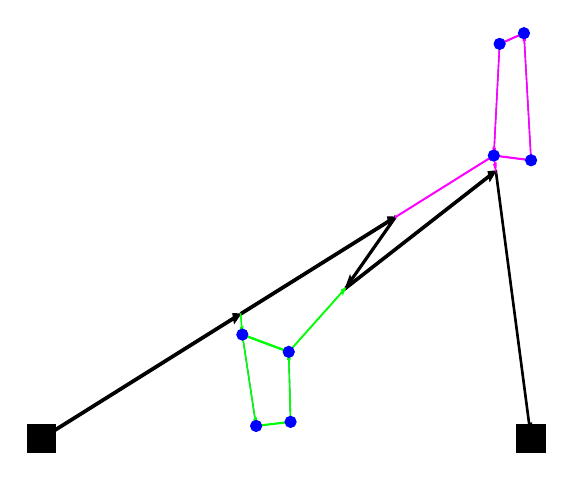
\begin{tikzpicture}[scale = 1]

\definecolor{color0}{rgb}{1,0,1}
\definecolor{color1}{rgb}{1,0.647058823529412,0}

\begin{axis}[
hide x axis,
hide y axis,
scaled x ticks=manual:{}{\pgfmathparse{#1}},
scaled y ticks=manual:{}{\pgfmathparse{#1}},
tick align=outside,
x grid style={white!69.0196078431373!black},
xmajorticks=false,
xmin=-5.05502235858009, xmax=105.174614066404,
xtick style={color=black},
xticklabels={},
y grid style={white!69.0196078431373!black},
ymajorticks=false,
ymin=-2.21430082601252, ymax=43.3494567401465,
ytick style={color=black},
yticklabels={}
]
\path [draw=blue]
(axis cs:92.3875096510917,28.760880398367)
--(axis cs:100,28.2794147343731);

\path [draw=blue]
(axis cs:92.3875096510917,28.760880398367)
--(axis cs:93.5775927984662,40.1087495102706);

\path [draw=blue]
(axis cs:100,28.2794147343731)
--(axis cs:98.5401123942739,41.1944465598056);

\path [draw=blue]
(axis cs:93.5775927984662,40.1087495102706)
--(axis cs:98.5401123942739,41.1944465598056);

\path [draw=blue]
(axis cs:43.8355352373253,1.27994935031229)
--(axis cs:50.8720803503274,1.6950600202796);

\path [draw=blue]
(axis cs:43.8355352373253,1.27994935031229)
--(axis cs:41.0205665640108,10.5650797543875);

\path [draw=blue]
(axis cs:50.8720803503274,1.6950600202796)
--(axis cs:50.499509990895,8.80716884051199);

\path [draw=blue]
(axis cs:41.0205665640108,10.5650797543875)
--(axis cs:50.499509990895,8.80716884051199);

\path [draw=black, fill=black]
(axis cs:40.6712279107997,12.661627094896)
--(axis cs:39.3876489420068,11.7383584282162)
--(axis cs:39.2836130498196,12.0725388183303)
--(axis cs:0.0445868109373961,-0.14322016719175)
--(axis cs:-0.0445868109373961,0.14322016719175)
--(axis cs:39.1944394279448,12.3589791527138)
--(axis cs:39.0904035357575,12.6931595428279)
--cycle;
\path [draw=black, fill=black]
(axis cs:72.2742653520524,22.4992894800669)
--(axis cs:70.9906627657779,21.5760536485974)
--(axis cs:70.8866354222085,21.9102366999179)
--(axis cs:40.7158110580437,12.5184057871872)
--(axis cs:40.6266447635556,12.8048484026048)
--(axis cs:70.7974691277204,22.1966793153355)
--(axis cs:70.693441784151,22.530862366656)
--cycle;
\path [draw=black, fill=black]
(axis cs:62.0843389713264,15.2704058105617)
--(axis cs:63.0184491135358,16.5461166877676)
--(axis cs:63.2209606877944,16.2606537964992)
--(axis cs:72.1874746773702,22.621630719182)
--(axis cs:72.3610560267347,22.3769482409519)
--(axis cs:63.3945420371589,16.0159713182692)
--(axis cs:63.5970536114175,15.7305084270008)
--cycle;
\path [draw=black, fill=black]
(axis cs:92.802004052626,27.1951748475345)
--(axis cs:91.5846209683839,26.1862256782493)
--(axis cs:91.457958458731,26.5125025677901)
--(axis cs:62.1386229040348,15.1305728579014)
--(axis cs:62.030055038618,15.4102387632221)
--(axis cs:91.3493905933141,26.7921684731108)
--(axis cs:91.2227280836612,27.1184453626516)
--cycle;
\path [draw=black, fill=black]
(axis cs:100,0)
--(axis cs:99.1328415665434,1.3221332199461)
--(axis cs:99.471190633074,1.41168716557576)
--(axis cs:92.6569973098271,27.1567945851218)
--(axis cs:92.9470107954248,27.2335551099472)
--(axis cs:99.7612041186717,1.48844769040119)
--(axis cs:100.099553185202,1.57800163603086)
--cycle;
\path [draw=green, fill=green]
(axis cs:41.0205665640108,10.5650797543875)
--(axis cs:40.6506966975442,11.2637901964735)
--(axis cs:40.8479767929622,11.2966621290586)
--(axis cs:40.6219078869452,12.6534091117497)
--(axis cs:40.7205479346541,12.6698450780423)
--(axis cs:40.9466168406712,11.3130980953511)
--(axis cs:41.1438969360891,11.3459700279363)
--cycle;
\path [draw=green, fill=green]
(axis cs:41.0205665640108,10.5650797543875)
--(axis cs:41.8035787828808,10.6741295829079)
--(axis cs:41.7671097642161,10.4774826640974)
--(axis cs:50.5086272455611,8.8563305702146)
--(axis cs:50.4903927362288,8.75800711080939)
--(axis cs:41.7488752548837,10.3791592046922)
--(axis cs:41.712406236219,10.1825122858818)
--cycle;
\path [draw=green, fill=green]
(axis cs:50.8720803503274,1.6950600202796)
--(axis cs:50.138104829191,1.40132555792856)
--(axis cs:50.1263265999177,1.60097843998936)
--(axis cs:43.8384797946437,1.23003612979709)
--(axis cs:43.832590680007,1.32986257082749)
--(axis cs:50.120437485281,1.70080488101976)
--(axis cs:50.1086592560077,1.90045776308056)
--cycle;
\path [draw=green, fill=green]
(axis cs:43.8355352373253,1.27994935031228)
--(axis cs:43.3786913106025,1.92515755439566)
--(axis cs:43.5700887937204,1.98318344048246)
--(axis cs:40.9727171932314,10.5505732828658)
--(axis cs:41.0684159347903,10.5795862259092)
--(axis cs:43.6657875352793,2.01219638352586)
--(axis cs:43.8571850183971,2.07022226961266)
--cycle;
\path [draw=green, fill=green]
(axis cs:50.499509990895,8.80716884051185)
--(axis cs:50.7884028865625,8.07127421841382)
--(axis cs:50.5886767456056,8.06081149322144)
--(axis cs:50.9220118855666,1.69767570157756)
--(axis cs:50.8221488150881,1.69244433898138)
--(axis cs:50.4888136751271,8.05558013062526)
--(axis cs:50.2890875341702,8.04511740543288)
--cycle;
\path [draw=green, fill=green]
(axis cs:50.499509990895,8.80716884051199)
--(axis cs:49.716497772025,8.69811901199165)
--(axis cs:49.7529667906897,8.89476593080208)
--(axis cs:41.0114493093446,10.5159180246849)
--(axis cs:41.029683818677,10.6142414840901)
--(axis cs:49.7712013000221,8.99308939020728)
--(axis cs:49.8076703186868,9.18973630901771)
--cycle;
\path [draw=green, fill=green]
(axis cs:62.0843389713264,15.2704058105617)
--(axis cs:61.5511779430038,14.6866770054836)
--(axis cs:61.4537359120508,14.8613339566872)
--(axis cs:50.5238704986332,8.76350460271093)
--(axis cs:50.4751494831567,8.85083307831277)
--(axis cs:61.4050148965743,14.9486624322891)
--(axis cs:61.3075728656214,15.1233193834928)
--cycle;
\path [draw=color0, fill=color0]
(axis cs:92.3875096510916,28.760880398367)
--(axis cs:91.7457202656468,28.2992459274592)
--(axis cs:91.6862711434645,28.4902061376385)
--(axis cs:72.289127632598,22.4515494275221)
--(axis cs:72.2594030715068,22.5470295326118)
--(axis cs:91.6565465823734,28.5856862427282)
--(axis cs:91.5970974601911,28.7766464529076)
--cycle;
\path [draw=color0, fill=color0]
(axis cs:100,28.2794147343731)
--(axis cs:99.2357154035718,28.0772537696382)
--(axis cs:99.2483395397497,28.2768549499598)
--(axis cs:92.3843536170472,28.7109801032866)
--(axis cs:92.3906656851361,28.8107806934474)
--(axis cs:99.2546516078387,28.3766555401206)
--(axis cs:99.2672757440165,28.5762567204421)
--cycle;
\path [draw=color0, fill=color0]
(axis cs:92.3875096510916,28.760880398367)
--(axis cs:92.2170988265126,29.5328649518823)
--(axis cs:92.4160079853226,29.5120047855001)
--(axis cs:93.5278655087637,40.1139645518661)
--(axis cs:93.6273200881687,40.103534468675)
--(axis cs:92.5154625647276,29.501574702309)
--(axis cs:92.7143717235376,29.4807145359267)
--cycle;
\path [draw=color0, fill=color0]
(axis cs:98.5401123942739,41.1944465598056)
--(axis cs:98.8727722475555,40.4772733436195)
--(axis cs:98.6740378874083,40.4548088361268)
--(axis cs:100.049683590037,28.2850308612462)
--(axis cs:99.9503164099632,28.2737986074999)
--(axis cs:98.5746707073347,40.4435765823804)
--(axis cs:98.3759363471875,40.4211120748878)
--cycle;
\path [draw=color0, fill=color0]
(axis cs:93.5775927984662,40.1087495102706)
--(axis cs:94.2568322432455,40.5132662301425)
--(axis cs:94.2995771004324,40.3178874258057)
--(axis cs:98.5294261799772,41.2432912608898)
--(axis cs:98.5507986085707,41.1456018587214)
--(axis cs:94.3209495290259,40.2201980236374)
--(axis cs:94.3636943862128,40.0248192193006)
--cycle;
\path [draw=color0, fill=color0]
(axis cs:92.802004052626,27.1951748475345)
--(axis cs:92.3683913862325,27.8562195173891)
--(axis cs:92.5617311203091,27.9074029837351)
--(axis cs:92.3391747175725,28.7480845317805)
--(axis cs:92.4358445846108,28.7736762649535)
--(axis cs:92.6584009873474,27.9329947169081)
--(axis cs:92.851740721424,27.9841781832542)
--cycle;
\addplot [draw=blue, fill=blue, mark=*, only marks]
table{%
x  y
92.3875096510917 28.760880398367
100 28.2794147343731
93.5775927984662 40.1087495102706
98.5401123942739 41.1944465598056
};
\addplot [draw=blue, fill=blue, mark=*, only marks]
table{%
x  y
43.8355352373253 1.27994935031229
50.8720803503274 1.6950600202796
41.0205665640108 10.5650797543875
50.499509990895 8.80716884051199
};
\addplot [semithick, black, mark=square*, mark size=5, mark options={solid}, only marks]
table {%
0 0
};
\addplot [semithick, black, mark=square*, mark size=5, mark options={solid}, only marks]
table {%
100 0
};
\end{axis}

\end{tikzpicture}
\caption{Feasible solution with partial overlapping that is not feasible for the complete overlapping model.}
\label{fig:proof2}
\end{figure}